\documentclass[a4paper,12pt]{report}
\usepackage{geometry}
 \geometry{
 a4paper,
 total={210mm,297mm},
 left=25mm,
 right=25mm,
 bottom=25mm,
 top=25mm,
 }
\usepackage[english]{babel}
\usepackage[T1]{fontenc}
\usepackage[utf8]{inputenc}
\usepackage{lmodern}
\usepackage{microtype}
\usepackage{graphicx}
\usepackage{caption} 
\usepackage{titling}
\usepackage[colorlinks=true,linkcolor=black,urlcolor=blue]{hyperref}
\usepackage{indentfirst}
\usepackage{siunitx}
\usepackage{amsmath}
\usepackage[backend=biber,]{biblatex}
\nocite{*}
\addbibresource{Biblio.bib}



\title{Bibliographical Project \\ [1ex]\large X-Rays and Radiography \\ (based on the work of Wilhem Röntgen)  }
\author{Ulysse MERAD\and Ruben LEGRANDJACQUES \and \\Fabrice LIN \and Anwar AL-BITAR}

\date{October 1, 2023} 

\begin{document}

\begin{titlepage}
  \centering
  \vspace{3cm}
  \Huge{\textbf{Bibliographical Project}}\\
  \vspace{1cm}
  \Large{X-Rays and Radiography \\ (based on the work of Wilhem Röntgen)} \\
  \vspace{0.5cm}
  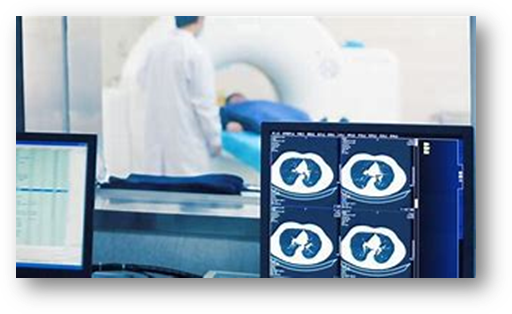
\includegraphics[scale=1]{xray.png}\\
  \vspace{0.5cm}
  Ulysse MERAD, Ruben LEGRANDJACQUES, \\ [0.5ex] Fabrice LIN, Anwar AL-BITAR \\
  \vspace{1.5cm}
  \large{\textit {Under the supervision of A.LEHMANN and F.MANDIJA}} \\
  \vspace{1.5cm}
  \thedate \\
  \vspace{2cm}
  
\includegraphics[scale=0.6]{Isep.jpg}\\
  
\end{titlepage}



\newpage

\tableofcontents
\addcontentsline{toc}{section}{Introduction}

\setlength{\parskip}{10pt}


\newpage
\section*{Introduction}

Before starting explanation of Wilhelm Röntgen's work and discovery we have made the choice of introduce a brief abstract on current theorical aspect of X-rays. There are several elementary points usefull to understand. Please keep in mind during lecture those notions.

\href{https://radiologymasterclass.co.uk}{Basics of X-ray Physics - X-ray production}\\ 

\href{https://www.britannica.com/biography/Wilhelm-Rontgen}{Wilhelm Conrad Roentgen | Biography, Discovery, X-Rays, \& Facts | Britannica }
\subsection*{Basics of X-rays's physics}
X-rays, also recognized as X-radiation, are a form of electromagnetic radiation characterized by
high energies. Radiation categorization is based on its wavelength \(\lambda\), representing the length of
one complete wave cycle. This wavelength can alternatively be defined in terms of frequency \(\nu\)
and the propagation speed of the wave, denoted as the speed of light. The relationship
between these parameters is fundamental in characterizing different types of radiation, illustrating
the interplay between wavelength, frequency, and the speed of light in the electromagnetic
spectrum.

\begin{equation}
  \lambda = \frac{c}{\nu}
\end{equation}


The energy of a photon is characterised by the following formula :

\[E= \frac{hc}{\lambda}= h\nu\]

The energy of photons can be expressed using Planck's constant \(h \approx 6.626.10^{-3} J.s\) and the
speed of light \(c \approx 2.997.10^8 m.s^{-1}\). This energy is directly connected to the wavelength \(\lambda\) or
frequency \(\nu\) of the photon, measured in electron volts [eV]. The relationship reveals that the
photon energy is directly proportional to its frequency and inversely proportional to its
wavelength. In simpler terms, an increase in frequency corresponds to higher energy, highlighting
the direct relationship between these fundamental properties of photons.

These high-energy photons possess short wavelengths, resulting in exceptionally high
frequencies. The pivotal parameter defining all photons is their radiation frequency, which, in
turn, determines their energy. Photons are classified based on their energies, spanning from low-
energy radio waves and infrared radiation, progressing through visible light, and culminating in
high-energy X-rays and gamma rays.
\newpage

Here is the complete electromagnetic spectrum :
\begin{center}
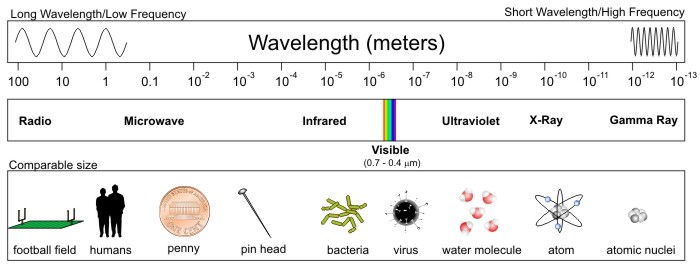
\includegraphics[scale = 2.4]{elecSpec.jpg}
\captionof{figure}{The Electromagnetic Spectrum}
\end{center}

It is relevant to note that \textit{X-rays and Gamma-rays} are also called \textit{ionizing radiation} meaning they have engough energy to transform atom they go through into ions. Hence, the atom loose or receive an electron. This can make matter unstable.

\subsection*{Bremsstrahlung effect or braking radiation}

In today's world, X-rays are generated using specialized X-ray machines. These machines offer
the flexibility to adjust both current and voltage settings, enabling the manipulation of the
properties of the X-ray beam produced. This capability allows for the application of distinct X-
ray beam spectra tailored to specific body parts during medical imaging procedures.

Nowadays, Science explains the generation of X-rays  the \textit{Bremsstrahlung }effect from the German, braking radiation. 


Maxwell's equations:
\begin{align}
  \nabla \cdot \vec{E} &= \dfrac{\rho}{\varepsilon_0} \\
  \nabla \cdot \vec{B} &= 0 \\
  \nabla \times \vec{E} &= -\dfrac{\partial \vec{B}}{\partial t} \\
  \nabla \times \vec{B} &= \mu_0 \vec{J} + \mu_0 \varepsilon_0 \dfrac{\partial \vec{E}}{\partial t}
\end{align}

Lorentz force equation:
\begin{equation}
  \vec{F} = q(\vec{E} + \vec{v} \times \vec{B})
\end{equation}






\chapter{Historical Background}
\section{Radiation Understanding in the Late 19\textsuperscript{th} century}
  Here we'll talk about the scientific and technological developments preceding Röntgen's work. We will also talk about the state of physics and understanding of radiation in the late 19th century. 

\chapter{Life and Career of Wilhelm Conrad Röntgen}
\section{Early Life of an enthusiastic genius}
Sometimes history is made of incredible destiny. Wilhelm Conrad Röntgen, born on March 27\textsuperscript{th}, 1845 near Dusseldorf, Germany was not incline to brillant physics studies. 
His father a sheet merchant did not push him throughout this way. Rôntgen's early life was marked by a move to Netherlands for his father's business.
\section{Röntgen's groundbreaking experiment}
First, we will do a quick biography of Wilhelm Conrad Röntgen's early life and education, his career progression and key influences. Then we will talk over how his background contributed to his groundbreaking work.~\footfullcite{NUSSLIN202065}\\
\href{https://www.sciencedirect.com/science/article/pii/S1120179720302532}{Wilhelm Conrad Röntgen: The scientist and his discovery - ScienceDirect }

\chapter{The Discovery of X-Rays}
\section{Impact of Röntgen's X-Rays discovery}
In this chapter we will reveal Röntgen's experimental setup and methodology, the moment of his discovery. Then we will show the first X-ray images, and the reaction of the public and scientific world after the discovery.
\section{Radiography's Early Applications and Pioners}
Here, we will dive thought on howRöntgen's discovery led to the development of radiography. We will also discuss about the pioneers in radiography who followed Röntgen We will finalize by talking about the early applications of radiography in medicine and industry.

\chapter{Advances  in Radiographic Technology}
\section{Evolution of Radiography Equipment and Techniques}
Here, we will talk about the evolution of radiographic equipment and techniques. 
\section{	Technological Breakthroughs in Radiography}
We will follow up by discussing technological breakthroughs in radiography. 
\section{Radiography During World War I and II}
We will extend this chapter by talking about the impact of World War I and World War II on radiography. 

\href{https://radiologykey.com/principles-of-radiography/}{Principles of radiography | Radiology Key, (radiographie) }

\href{https://www.ramsoft.com/history-of-radiology/}{History of Radiology: Timeline, Pioneers, Inventions | RamSoft  }

\chapter{Modern Applications of Radiography}
\section{Contemporary Uses and Challenges in Radiography}
We will emphasize here the contemporary uses of radiography in medicine, industry, and other fields, along with the benefits and challenges of modern radiographic technology.
\href{https://healthmanagement.org/c/healthmanagement/issuearticle/radiology-in-2020-opportunities-and-challenges#:~:text=%E2%80%A2%20Radiological%20technology%20is%20shifting%20from%20a%20%E2%80%9Cdisruptive%E2%80%9D,In%20vitro%20diagnostics%20will%20change%20radiological%20screening%20policy.}{Radiology in 2020: Opportunities and Challenges - HealthManagement.org }


\chapter{Ethical and Safety Considerations in Radiography}

\section{Ethical and Safety issues in Radiography}
We will talk about ethical and safety issues related to radiographic procedures\\
\href{https://www.ncbi.nlm.nih.gov/books/NBK232703/}{History of Radiation Regulation in Medicine - Radiation In Medicine - NCBI Bookshelf (nih.gov)}\\
\href{https://hbr.org/sponsored/2022/10/5-imperatives-for-radiation-dose-management-in-medical-imaging}{5 Imperatives for Radiation Dose Management in Medical Imaging  (hbr.org)}
\section{Development of Safety Protocols and Regulations}
In this chapter we will discuss the development of safety protocols and regulations, along with the importance of radiation dose management.

\href{https://www.britannica.com/science/radiation/Artificial-sources}{Radiation - Artificial Sources | Britannica ( affects of radiation on body with charts)}

\chapter{Wilhem Conrad Röntgen's Legacy}
\section{Importance of Radiation Dose Management}
\section{Lasting Impac and Legacy Röntgen}
\section{Recognition and Honors for Röntgen}
In this chapter we will talk about the lasting impact of Röntgen's work on X-rays and radiography. Then we will see the recognition and honours he received, and how his legacy continues to influence the field.

\chapter{Future Trends in Radiography}
\section{Future advancements in Radiography}
\section{Emerging Technologies and AI in Radiography}
Here we will discuss and argue about the potential advancements and innovations in radiography. The emerging technologies and applications in the field, and the role and influence that of artificial intelligence could have inradiography.
\href{https://www.sciencedirect.com/science/article/abs/pii/S107881742100095X}{Artificial intelligence in radiography: Where are we now and what does the future hold? - ScienceDirect }
\chapter{Conclusion}

- Summarize the key findings and contributions discussed in the essay.
- Reflect on the enduring significance of Wilhelm Conrad Röntgen's work.
- Discuss the ongoing and future relevance of radiography in various fields.



\printbibheading
- List all the sources usedin your research and writing, following a specific citation style (e.g., APA, MLA).\\[1ex]

\textbf{A real references numerotation system will be implemented, the use of  \LaTeX\ is really powerful for that. At the moment we only have link included in each section. We are aware of the necessity to have exhaustive and clear references for our work. }\\[1ex]


\printbibliography[type=book,heading=subbibliography,title={Books}]
\printbibliography[type=article, heading=subbibliography, title={Articles}]
\printbibliography[type=online,heading=subbibliography, title={Online Resources}]
\printbibliography[type=misc, heading=subbibliography, title={Other Documents}]
\appendix
\section*{\Huge{appendix}}
\addcontentsline{toc}{section}{Appendix}
- Include supplementary materials, such as additional images, charts, or data.\\
- Include the reproduction of the letter of Poincaré in the appendix. We may quote it some part as a whitness and illustrate the report with this piece of history. \footfullcite{PoincaréToRontgen}\\
- Jacques Nicolle is a brillant physicist that have produce very interesting researches on the work of several Physicists. His work his very usefull for us.
\section*{General Remarks}
\addcontentsline{toc}{section}{General Remarks}
Ensure thorough research and critical analysis throughout the essay. Maintain proper citation and adhere to the chosen citation style guidelines. Ensure a logical flow and coherence in the essay as you transition between chapters and sections.
\end{document} 
